\documentclass[a4paper,12pt]{article} % добавить leqno в [] для нумерации слева
\usepackage[a4paper,top=1.3cm,bottom=2cm,left=1.5cm,right=1.5cm,marginparwidth=0.75cm]{geometry}
%%% Работа с русским языком
\usepackage{cmap}					% поиск в PDF
\usepackage[warn]{mathtext} 		% русские буквы в фомулах
\usepackage[T2A]{fontenc}			% кодировка
\usepackage[utf8]{inputenc}			% кодировка исходного текста
\usepackage[english,russian]{babel}	% локализация и переносы
\usepackage{physics}
\usepackage{multirow}
\usepackage{bm}
\usepackage{longtable}
\usepackage{amsmath}

%%% Нормальное размещение таблиц (писать [H] в окружении таблицы)
\usepackage{float}
\restylefloat{table}


\usepackage{graphicx}

\usepackage{wrapfig}
\usepackage{tabularx}

\usepackage{hyperref}
\usepackage[rgb]{xcolor}
\hypersetup{
	colorlinks=true,urlcolor=blue
}
\usepackage{pgfplots}
\pgfplotsset{compat=1.9}
%%% Дополнительная работа с математикой
\usepackage{amsmath,amsfonts,amssymb,amsthm,mathtools} % AMS
\usepackage{icomma} % "Умная" запятая: $0,2$ --- число, $0, 2$ --- перечисление

%% Номера формул
%\mathtoolsset{showonlyrefs=true} % Показывать номера только у тех формул, на которые есть \eqref{} в тексте,

%% Шрифты
\usepackage{euscript}	 % Шрифт Евклид
\usepackage{mathrsfs} % Красивый матшрифт

%% Свои команды
\DeclareMathOperator{\sgn}{\mathop{sgn}}

%_\textup{ис} - для русских формул

%%% Заголовок
\author{Самойлов Михаил Б06-205}
\title{Лабораторная работа 3.7.3 \\
	\textbf{Изучение длинной линии}}
\date{\today}


\begin{document}
\maketitle	

\section{Цель работы}

 \begin{itemize}
     \item ознакомиться и проверить на практике теорию распространения электрических сигналов вдоль длинной линии
     \item измерить амплитудо- и фазово-частотные
	характеристики коаксиальной линии
     \item определить погонные характеристики такой линии
     \item на примере модели длинной линии изучить вопрос распределения амплитуды колебаний сигнала по длине линии.
 \end{itemize}
 \section{Оборудование}

	В работе используются: 
 \begin{itemize}
     \item осциллограф АКТАКОМ ADS-6142H
     \item генератора АКИП 3420/1
     \item бухта с коаксиальным кабелем pk 50-4-11
     \item схематический блок "модель длинной линии"
     \item магазин сопротивления Р33
     \item соединительные провода
 \end{itemize}

\section{Введение}
Удельная индуктивность единицы длины коаксиального кабеля, состоящего из тонкого сплошного цилиндрического проводника радиусом $r_1$ на оси изолированного коаксиального элемента радиусом $r_2$, между которыми проложена сплошная среда с диэлектрической проницаемостью $\epsilon$ и магнитной восприимчивостью $\mu$, выражается следующим образом:

\begin{equation}
    L_x = \frac{dL}{dx} = 2\mu ln \frac{r_2}{r_1}
\end{equation}

Формула, составляющая общую удельную ёмкость единицы длины кабеля, представлена ниже: 

\begin{equation}
    C_x = \frac{dC}{dx} = \frac{\epsilon}{2ln\frac{r_2}{r_1}}
\end{equation}

На концах элемента dx возникает падение напряжения в результате появления ЭДС индукции и существованием омического сопротивления проводников. обратно пропорционального удельной проводимости $\sigma$, а также разность токов, связанная с тем, что часть заряда перетекает на заряженные элементы кабеля:

\begin{equation}
\begin{cases}
    U(x) = U(x+dx)+\frac{L_xdx}{c^2}\frac{\partial I}{\partial t} + R_xdxI\\
    I(x) = I(x+dx)+\frac{\partial q}{\partial t}
\end{cases}
\end{equation}

Эта система называется системой телеграфных уравнений. Дифференцируя её один и второй раз, можно получить каноническое уравнение вида:

\begin{equation}
    \frac{\partial^2 U}{\partial t^2} - V_\text{Ф}^2 \frac{\partial^2 U}{\partial x^2} + \gamma \frac{\partial U}{\partial t} = 0
\end{equation}

, где фазовая скорость $V_\text{Ф}$ = $\frac{c}{\sqrt{L_xC_x}} = \frac{c}{\sqrt{\mu \epsilon}}$ (это получается при подстановке значений удельной ёмкости и индуктивности элемента), и декремент затухания $\gamma = R_xC_xV_\text{Ф}^2$ = $(C_xV_\text{Ф}^2)/\sigma S$. Решая каноническое уравнение, можно получить выражение для зависимости тока от координаты в проводе и напряжения на нагрузке в конце линии от времени:

\begin{equation}
    I(x, t) = U_0 \frac{C_xw}{k+i\alpha}e^{iwt}e^{(-\alpha + ik)x}
\end{equation}

\begin{equation}
    U_n(t) = U_0*e^{-\alpha l}e^{ikl}e^{-iwt}
\end{equation}

Здесь волновое число k = $w / V_\text{Ф}$, где w - частота сигнала, $\alpha$ – коэффициент затухания. При этом если согласовать нагрузку с длинной линией так, чтобы эта нагрузка воспринималась её бесконечным продолжением, т.е. выставить $R_0 = \sqrt{L_x} / c\sqrt{C_x}$, то напряжение в конце длинной линии будет выражаться формулой $U_H(t) = U_0e^{-\alpha I}$. Набег фазы при таком сопротивлении будет равен $\Delta \varphi$ = kl. Из последних двух выражений однозначно выражаются волновое число k и коэффициент затухания $\alpha$. 



 \subsection*{Экспериментальная установка}
   \begin{wrapfigure}{hr}{0.5\textwidth}
  \vspace{-20pt}
  \begin{center}
    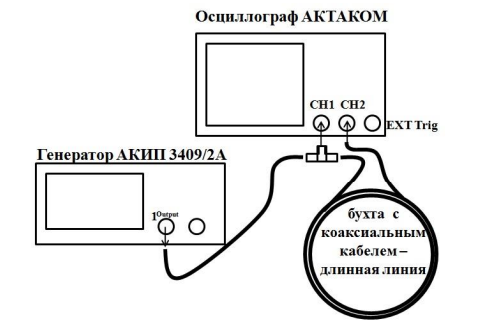
\includegraphics[width=0.5\textwidth]{plot/pic2.png}
    \caption{Схема экспериментальной установке}
  \end{center}
  \vspace{-10pt}
\end{wrapfigure}
 	Коаксиальный кабель подключается к генератору и осциллографу. На канал 1 выводится сигнал, подаваемый генератором, а с канала 2 снимается напряжение на нагрузке. Схема экспериментальной установки изображена ниже.

\clearpage

 
\section{Практическая часть}
\subsection{Оценка вазовой и групповой скорости}
В этой части работы будем определять резонансные частоты для синусоидального (СС) и прямоугольного (ПС) сигналов с нагрузкой, соответствующей согласованной линии и без нагрузки. 
Для синусоидального сигнала резонансные частоты численно соответствуют сдвигу фаз на 2$\pi$, откуда можно получить выражение

\begin{center}
   \large{$v_n = \frac{V_\text{Ф}}{l} (n+n_0)$}
\end{center}
откуда можно получить фазовую скорость из углового коэффициента линейной зависимости резонансной частоты от её номера. Численные результаты эксперимента приведены ниже:

\begin{table}[H]
    \centering
    \begin{tabular}{|c|c|c|c|c|c|c|c|} \hline
         n& 1 & 2 & 3 & 4 & 5 & 6 & 7\\ \hline
         $v_n \text{, (согласованная линия) МГц}$& 3.9 & 7.8 & 11.7 & 15.7 & 19.6 & 23.5 & 27.5\\ \hline
         $v_n \text{, (без нагрузки) МГц}$& 4 & 8 & 12 & 16 & 20 & 24 & 28\\ \hline
    \end{tabular}
    \caption{Результаты определения резонансных частот для синусоидальных колебаний.}
\end{table}

\begin{figure}[ht]
    \centering
    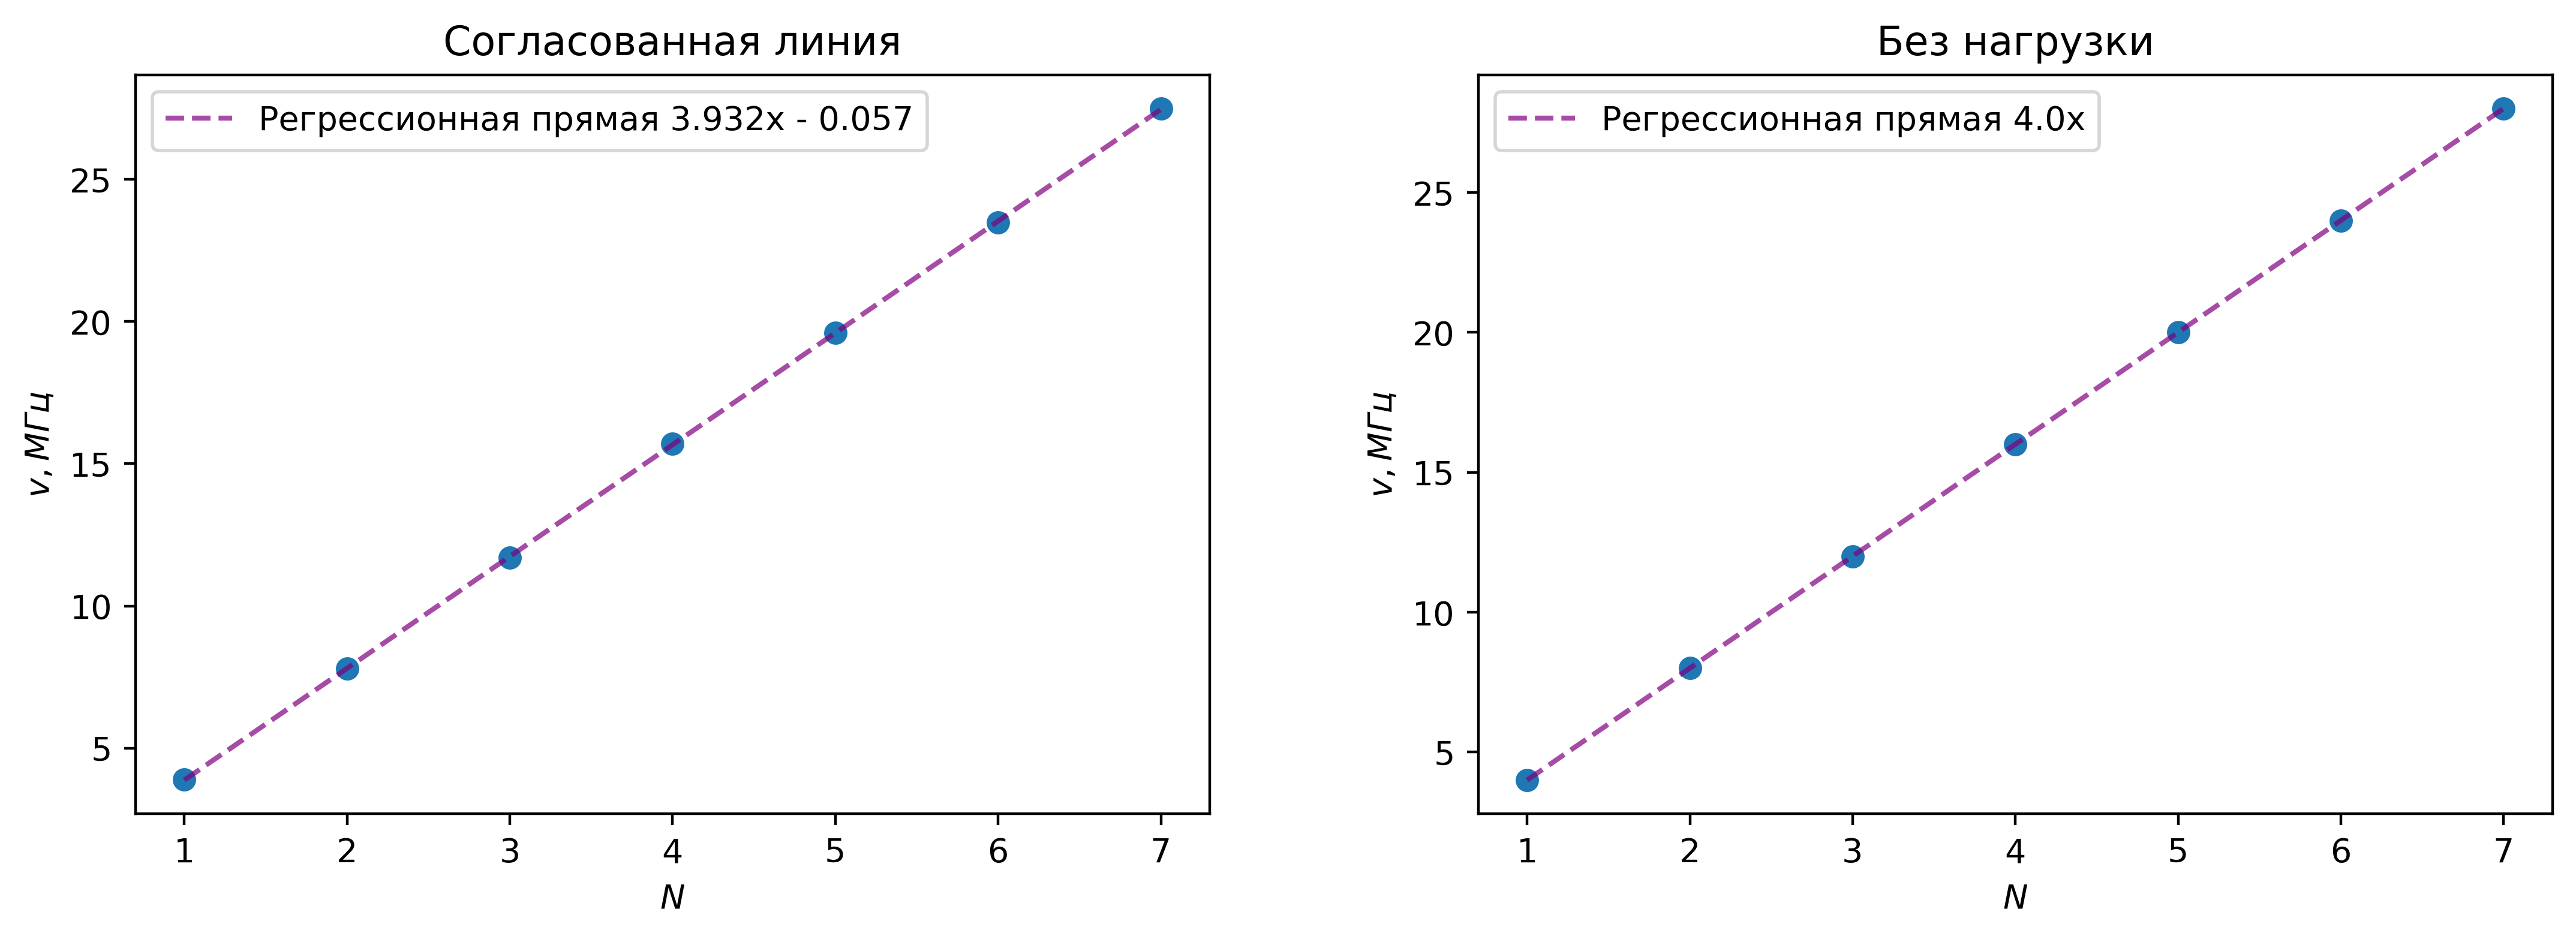
\includegraphics[width=1\linewidth]{plot/fig1.png}
    \caption{График зависимости резонансных частот от их номера для синусоидальных сигналов.}
\end{figure}

Среднеквадратичная ошибка для согласованной линии (с ее линнеаризацией) составила:
\begin{center}
    sd = 0.028
\end{center}

Из ошибки линейной аппроксимации, не превыщающей относительную погрешность измерения можно сделать вывод о почти нулевой дисперсии (что и видно из среднеквадратичной ошибки). Из графика по данным с согласованной нагрузкой можно получить информацию о угле наклона и фазовой скорости.

\begin{center}
    $k_1 = \frac{V_\text{Ф}}{l} = (4 \pm 0.003) \text{ МГц}$ \\
    $V_\text{Ф} = (2.012 \pm 0.002) * 10^{10} \text{ см/с}$
\end{center}

А для сигнала без нагрузки:
\begin{center}
    $k_2 = \frac{V_\text{Ф}}{l} = (3.93 \pm 0.006) \text{ МГц}$ \\
    $V_\text{Ф} = (1.977 \pm 0.003) * 10^{10} \text{ см/с}$
\end{center}


Для прямоугольного сигнала будет наблюдаться резонанс, когда сдвиг между сигналами равен $\Delta t = l / V_\text{групповая}$ на входе и выходе будет совпадать или кратен периоду подачи этих сигналов $T = (n + n_0)(1 / v_n)$

Из этого равенства можно получить выражение для зависимости резонансной частоты от её номера, из углового коэффициента которой однозначно получается значение групповой скорости:

\begin{center}
    \large{$v_n = \frac{V_\text{гр}}{l} (n + n_0)$}
\end{center}

Приведем данные и график полученный по этим данным

\begin{table}[H]
    \centering
    \begin{tabular}{|c|c|c|c|c|c|} \hline
         n & 1 & 2 & 3 & 4 & 5\\ \hline
         $v_n \text{, (согласованная линия) МГц}$& 3.92 & 7.82 & 11.74 & 15.65 & 19.59\\ \hline
         $v_n \text{, (без нагрузки) МГц}$& 3.9 & 7.8 & 11.7 & 15.7 & 19.5\\ \hline
    \end{tabular}
    \caption{Данные для прямоугольного сигнала}
\end{table}

\begin{figure}[H]
    \centering
    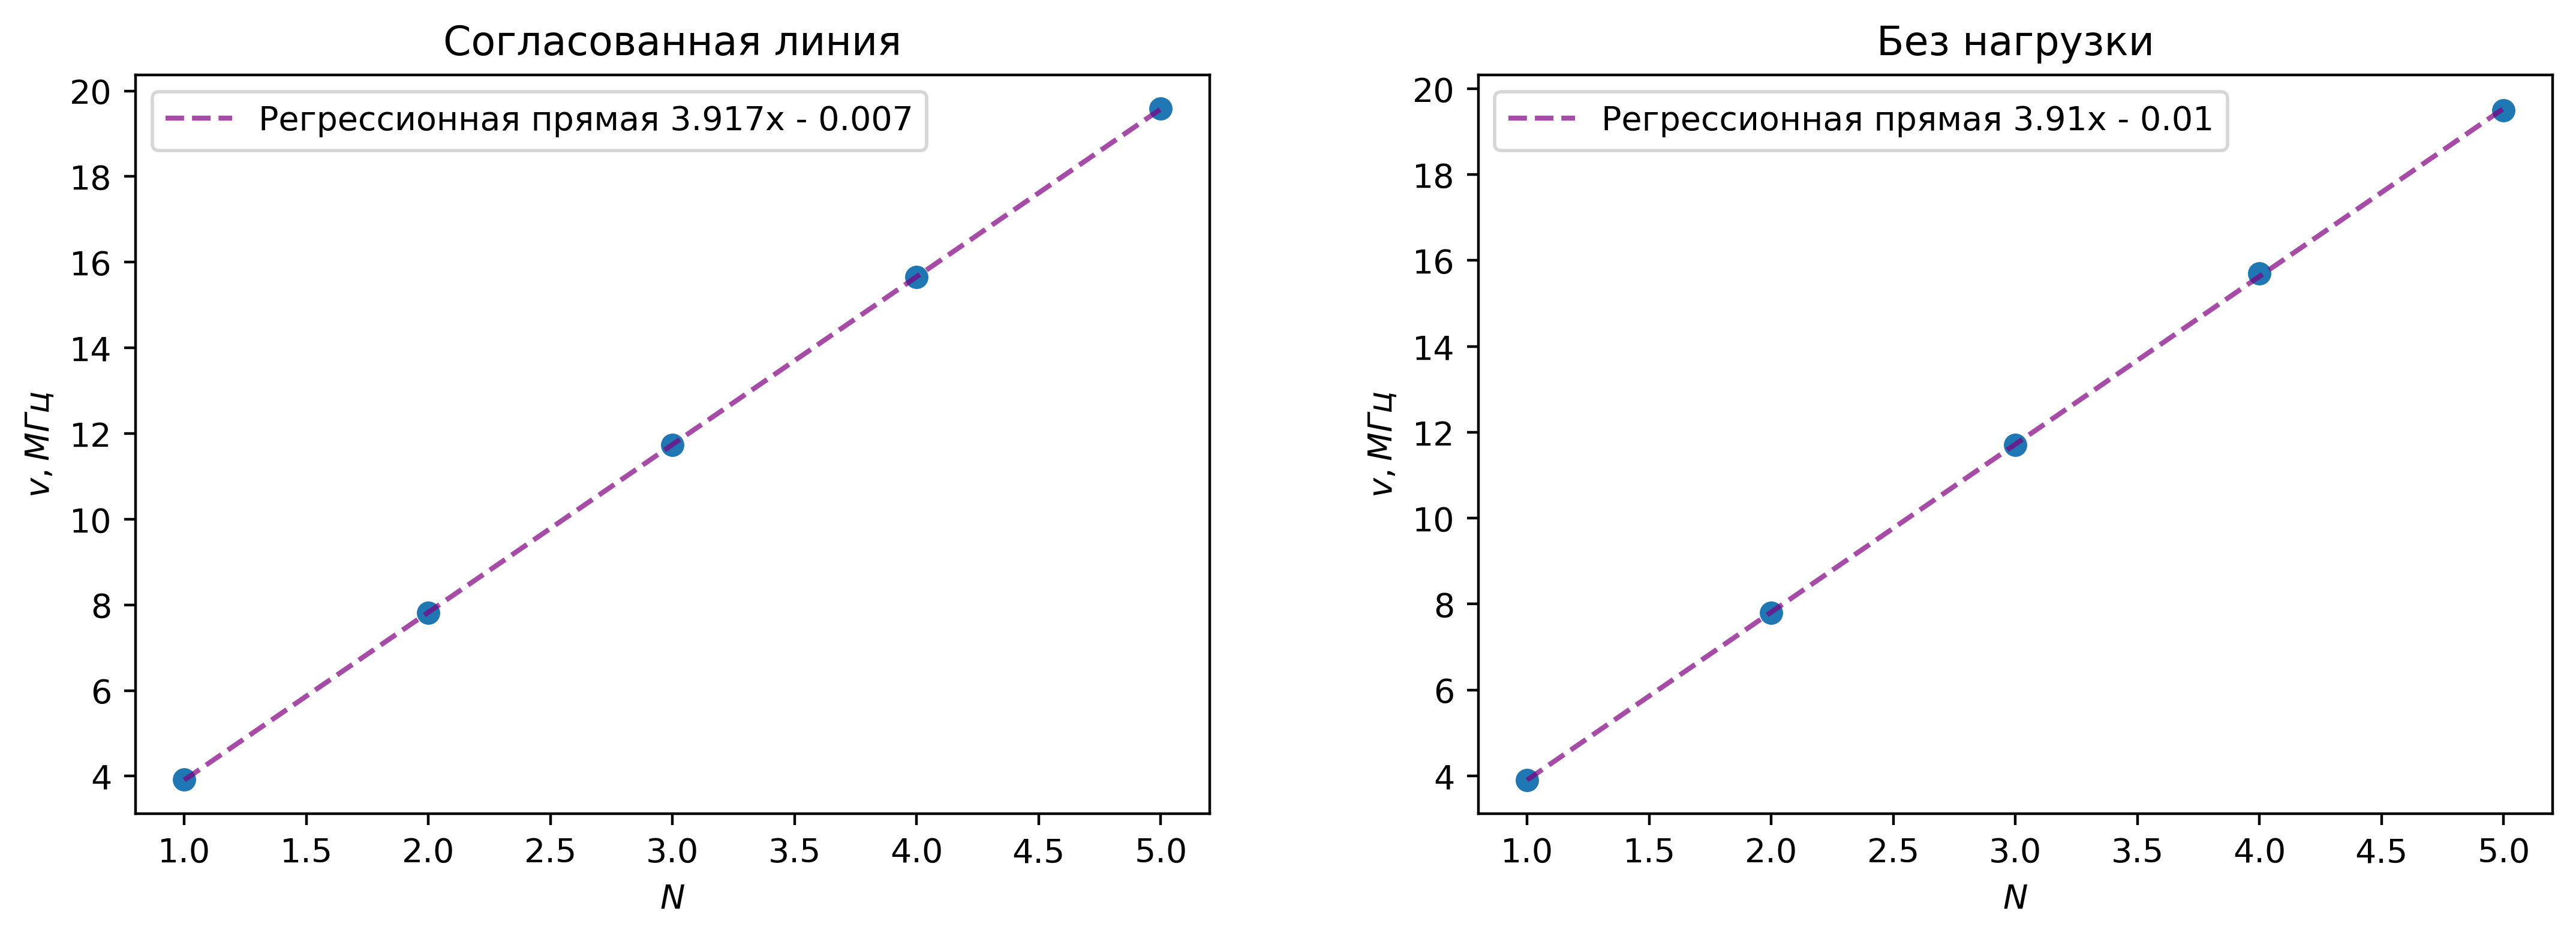
\includegraphics[width=1\linewidth]{plot/fig2.png}
    \caption{График зависимости резонансных частот от их номера для прямоугольных сигналов.}
\end{figure}

Для данных графиков получаем приведенные значения снизу. Для согласованной линии получаем:
\begin{center}
    $k_1 = \frac{V_\text{Ф}}{l} = (3.917 \pm 0.003) \text{ МГц}$ \\
    $V_\text{Ф} = (1.97 \pm 0.02) * 10^{10} \text{ см/с}$
\end{center}

А для сигнала без нагрузки:
\begin{center}
    $k_2 = \frac{V_\text{Ф}}{l} = (3.91 \pm 0.002) \text{ МГц}$ \\
    $V_\text{Ф} = (1.966 \pm 0.02) * 10^{10} \text{ см/с}$
\end{center}

\subsection{Амплитудно-частотные и фазово-частотные характеристики.}

Построим амплитудно-частотные (снимая амплитуду с первого канала в начале длинной линии и второго в её конце) и фазово-частотные (для сдвига фаз двух каналов друг относительно друга) характеристики кабеля на согласованной нагрузке. Для каждой частоты также определим коэффициент затухания и волновое число, исходя из полученных в теоретической части формул для набега фаз $\Delta \varphi$ и амплитуд в начале и конце линии $U_0$ и $U_H$:

\begin{equation}
    \alpha(w) = \frac{a}{l} ln(\frac{U_0}{U_H})
\end{equation}

\begin{equation}
    k(w) = \frac{\Delta \varphi}{l}
\end{equation}


\begin{table}[H]
    \centering
    \begin{tabular}{|c|c|c|c|c|c|} \hline
    $v$, \text{МГц} & $U_0$, \text{МГц} & $U_H$, \text{МГц} & $\Delta \varphi$, \text{рад} & $k$, $10^{-3}$ \text{см$^{-1}$} & $\alpha$, $10^{-3}$ \text{см$^{-1}$} \\ \hline
        1.0 & 54.0 & 50.8 & 2.87624 & 0.57182 & 0.01214 \\ \hline 
        2.0 & 53.9 & 49.6 & 5.57664 & 1.10868 & 0.0169 \\ \hline 
        3.0 & 53.9 & 48.8 & 5.12448 & 1.01878 & 0.02013 \\ \hline 
        4.0 & 54.0 & 48.4 & 5.19984 & 1.03377 & 0.02177 \\ \hline 
        7.0 & 54.0 & 46.0 & 10.06684 & 2.00136 & 0.03188 \\ \hline 
        9.0 & 54.0 & 45.0 & 13.33872 & 2.65183 & 0.03625 \\ \hline 
        12.0 & 53.9 & 43.6 & 15.61459 & 3.10429 & 0.04253 \\ \hline 
        15.5 & 54.1 & 41.2 & 19.70162 & 3.91682 & 0.05379 \\ \hline 
        19.0 & 54.0 & 40.8 & 24.7947 & 4.92936 & 0.05579 \\ \hline 
        22.5 & 53.9 & 39.6 & 29.87082 & 5.93853 & 0.06166 \\ \hline 
        26.0 & 54.0 & 38.8 & 34.94192 & 6.9467 & 0.06572 \\ \hline 
        31.0 & 54.0 & 36.0 & 39.61738 & 7.87622 & 0.08061 \\ \hline 
        36.0 & 53.9 & 34.2 & 46.36901 & 9.21849 & 0.09081 \\ \hline 
        40.0 & 54.0 & 33.2 & 51.42064 & 10.22279 & 0.09671 \\ \hline 
    \end{tabular}
    \caption{Основные данные секции Б}
\end{table}

\begin{figure}[H]
    \centering
    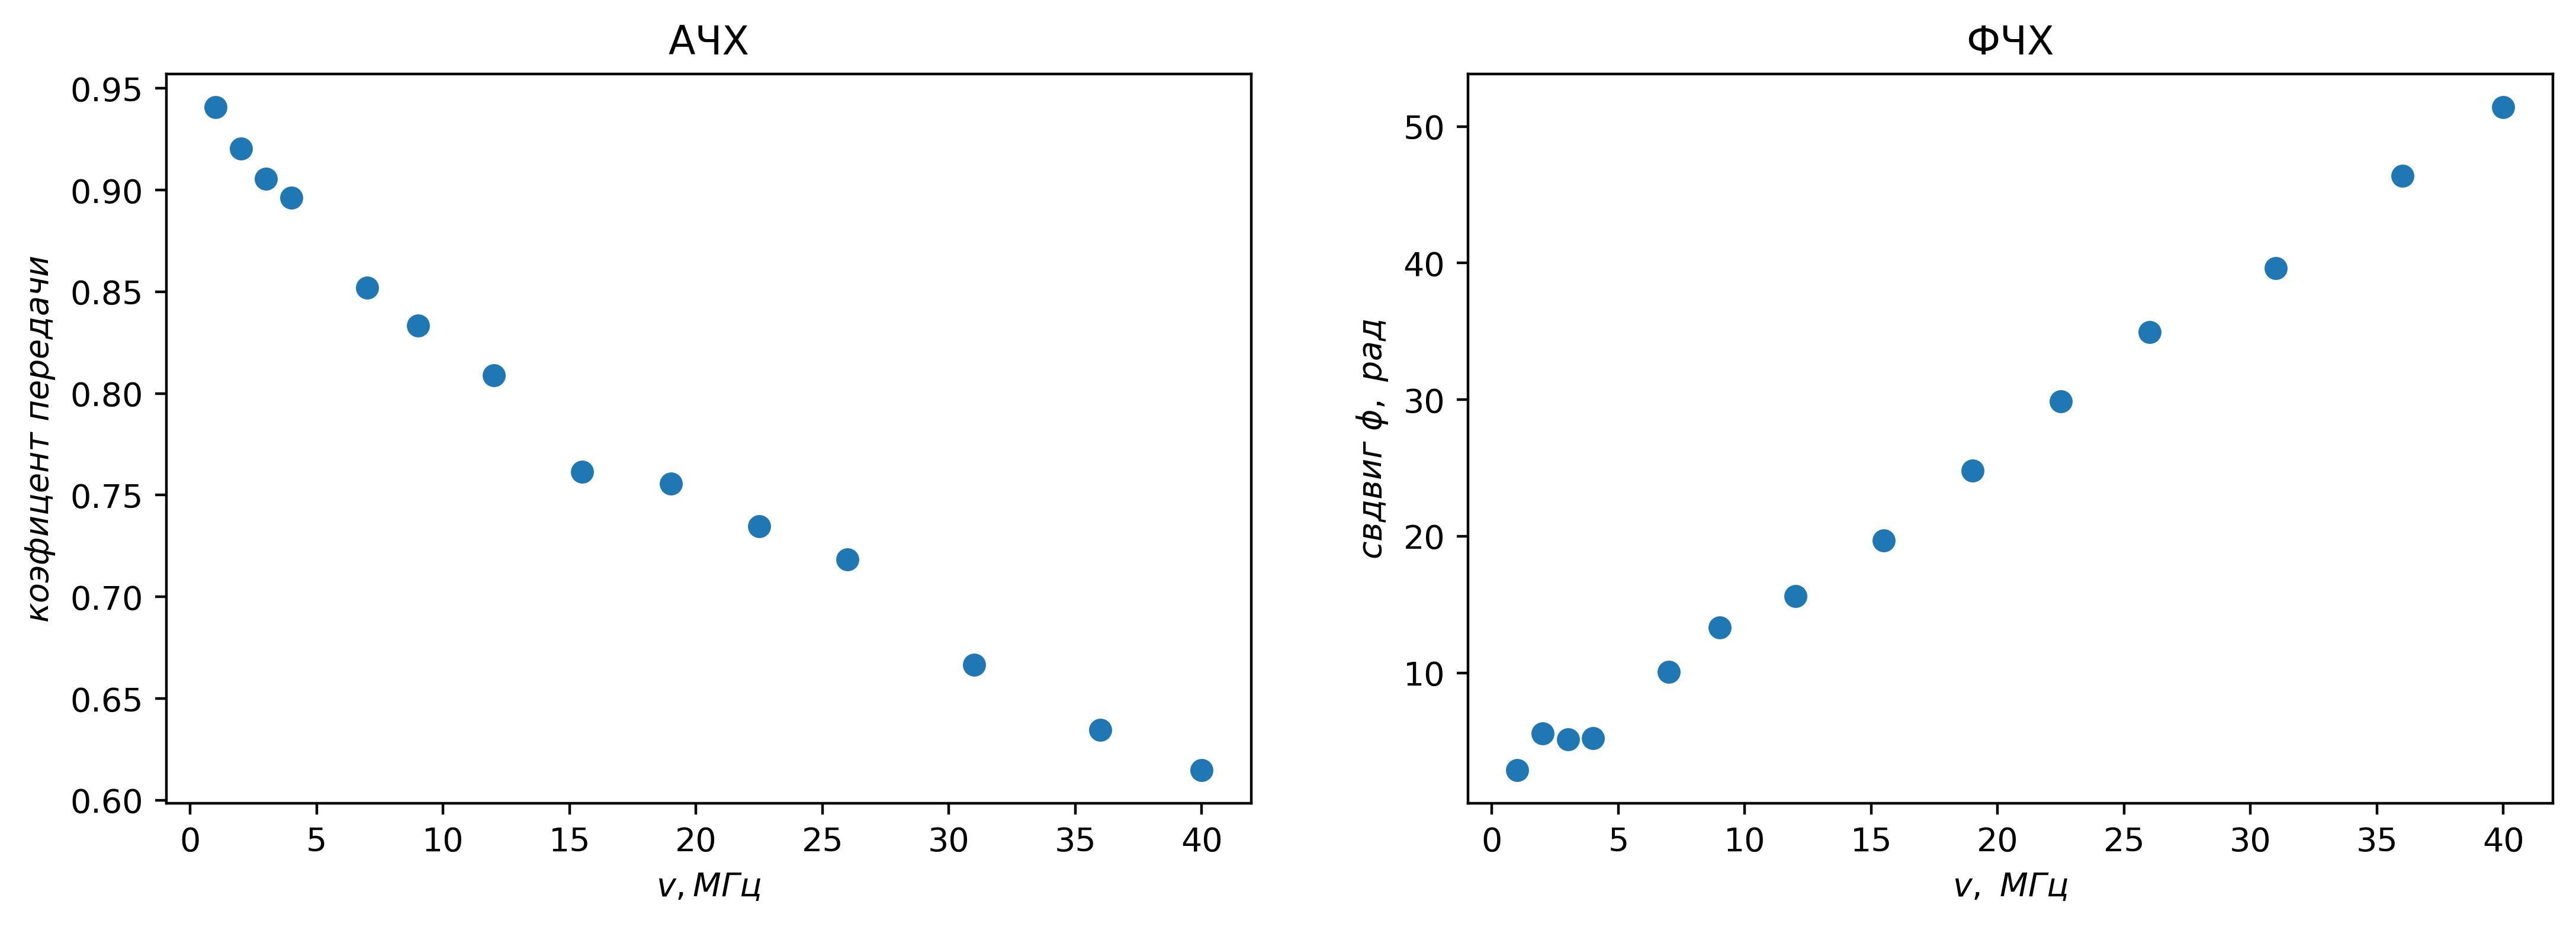
\includegraphics[width=1\linewidth]{plot/fig8.png}
    \caption{АЧХ и ФЧХ для наших данных.}
\end{figure}

Погрешности составляют $\sigma_v$ = 1 кГц,  $\sigma_U$ = 0.1 В. Для исследования АЧХ и ФЧХ используем решение канонического уравнения, находя его в виде двойной экспоненты. Разделив мнимую и действительную части полученного подстановкой выражения, наблюдаем следующее (система Х):

\begin{equation}
\begin{cases}
    w^2 = V_\text{Ф}^2 (k^2 - \alpha ^2) \\
    2\alpha kV_\text{Ф}^2 = w\gamma
\end{cases}
\end{equation}

На следующем графике построим зависимость $(k^2 - \alpha ^2)(w^2)$, учитывая что $w^2 = V_\text{Ф}^2 (k^2 - \alpha ^2)$, а значит угловой коэфицент полученного графика получится $(C_xL_x)/c^2$. Построим же этот график. 

\begin{figure}[H]
    \centering
    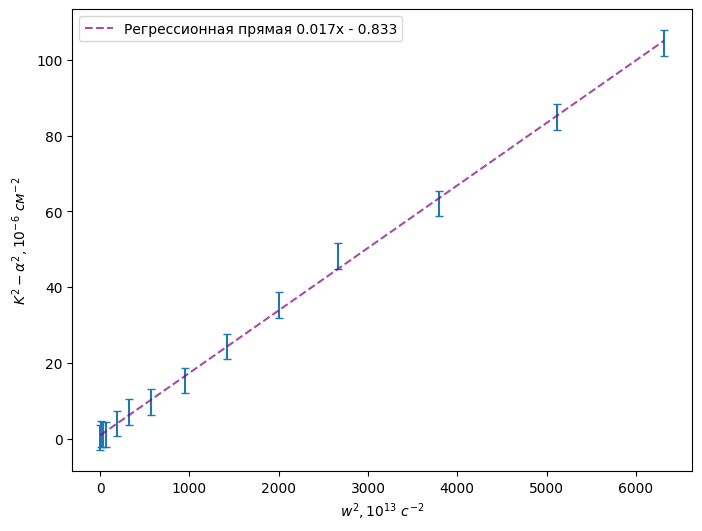
\includegraphics[width=0.7\linewidth]{plot/fig3.png}
    \caption{График зависимости $(k^2 - \alpha ^2)(w^2)$}
\end{figure}

По данному графику получаем значения:

\begin{center}
    $L_xC_x = (1.52 \pm 0.04)$
\end{center}

В нашем случае $R_0$ равно 50 Ом, так что можно написать соотношения $L_x = cR_0 = (2.05 \pm 0.03) \text{ ед СГС}, C_x = (0.74 \pm 0.02) см$. Фазовая скорость же равна $V_\text{Ф} = (2.43\pm0.07) * 10^{10}$ см/с. Данное значение сходится с полученным в первом пункте с погрешностью 28\%. Зная, что r1/r2 = 2.92, можно получить $\epsilon = 1.58 \pm 0.04 \text{ и } \mu = 0.96 \pm 0.03$

\subsection{Определение удельной проводимости проводников.}
\subsubsection{Метод А}
Можем связать параметры данным уравнением
\begin{equation}
    \alpha(w) = \frac{1}{l}ln(\frac{U_0}{U_H}) = \frac{4}{\sqrt{\sigma} d} C_x\frac{V_\text{Ф}}{c}\sqrt{v}
\end{equation}

А значит, построив график $\alpha(\sqrt{v})$ сможем по наклону предполагаемой прямой на графике определить $\sigma$.

\begin{figure}[H]
    \centering
    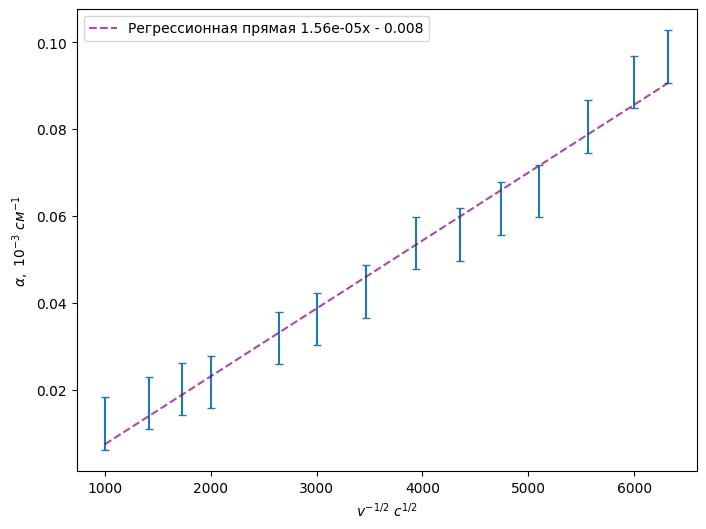
\includegraphics[width=0.7\linewidth]{plot/fig4.png}
    \caption{График для первого метода определения $\sigma$}
\end{figure}

Получаем значение
\begin{center}
    $\sigma = (1.06 \pm 0.04) * 10^{18}$
\end{center}

\subsubsection{Метод Б}
Для данного метода построим зависимость $\alpha k \text{ от }v^{3/2}$, чтобы из углового коэфицента определить $\sigma$.

\begin{figure}[H]
    \centering
    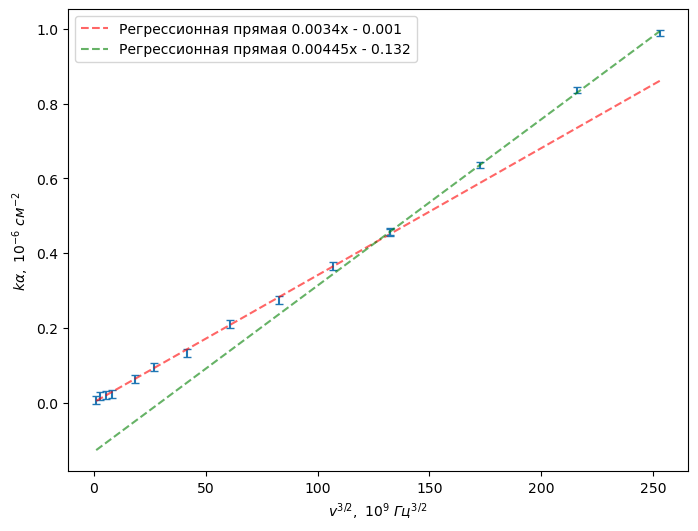
\includegraphics[width=0.7\linewidth]{plot/fig5.png}
    \caption{График для второго способа определения $\sigma$}
\end{figure}

Используя (25) и тот факт, что можно заменить декремент затухания, исходя из $\gamma = R_xC_xV_\text{Ф}^2$ получаем соотношение $2\alpha k = wR_xC_x$. Зная угловой коэфицент мы могли бы оценить $\sigma$, но данные выровнялись на 2 прямые. Значит, получим 2 значения $\sigma$:
\begin{center}
    $\sigma_{left} = (4.56 \pm 0.18) * 10^{17}$\\
    $\sigma_{right} = (2.99 \pm 0.11) * 10^{17}$
\end{center}
Это значение в пару раз меньше полученного прошлым методом.



\subsection{Модель длинной волны}
\begin{figure}[H]
    \centering
    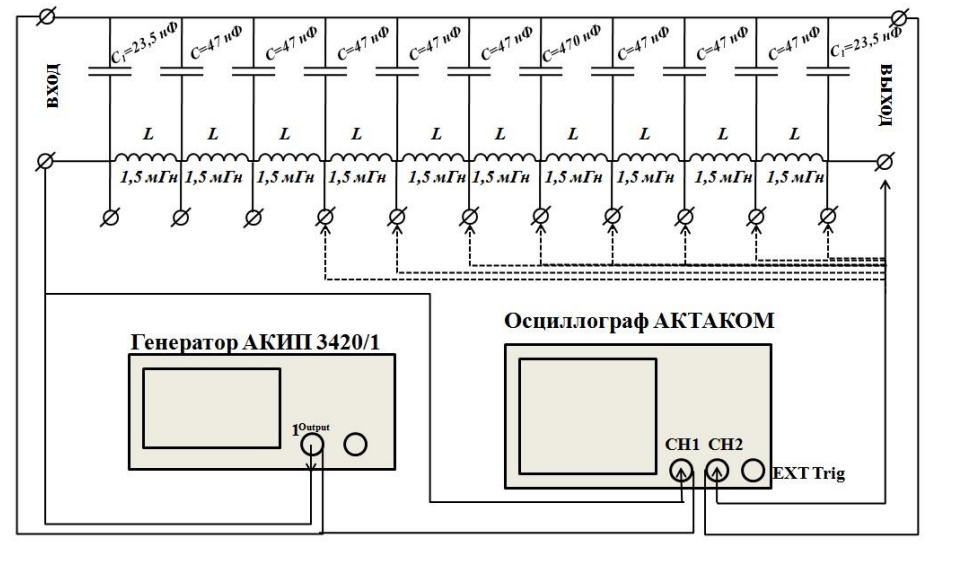
\includegraphics[width=0.7\linewidth]{plot/pic3.png}
    \caption{Используемая в работе установка}
\end{figure}

Прежде, чем приступить к работе определим предельную частоту распространения сигнала $v_0 = 1/\pi\sqrt{LC}$ = 38 кГц, согласованную нагрузку $R_0 = \sqrt{L/C}$ = 178 Ом. Теперь приведем экспериментальные данные.


\begin{table}[H]
    \centering
    \begin{tabular}{|c|c|c|c|c|c|c|c|c|c|c|c|} \hline
         v, кГц& 1 & 3 & 6 & 10 & 15 & 20 & 23 & 24 & 27 & 30 & 33\\ \hline
         $\Delta \varphi$& 6.34 & 16.77 & 32.21 & 50.83 & 78.94 & 101.2 & 118.6 & 122.9 & 136.0&154.0&166.0\\ \hline
    \end{tabular}
    \caption{Данные  по длинной волне}
\end{table}

Из теоретических формул можно вывести, что коэфицент наклона графика должен быть равен $2\pi/\epsilon_0$ = 5.96*$10^{-3}c^{-2}.$ Построим график и получим свой коэфицент наклона. 


\begin{figure}[H]
    \centering
    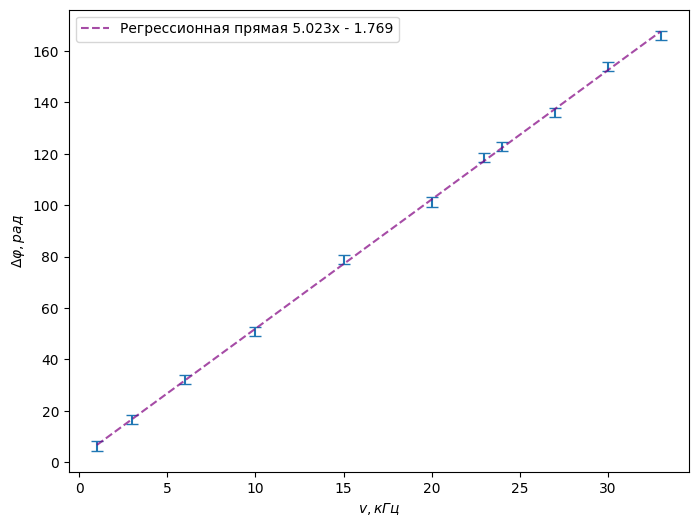
\includegraphics[width=0.7\linewidth]{plot/fig6.png}
    \caption{График зависимост сдвига фаз в ячейке от частоты сигнала}
\end{figure}

Угловой коэфицент составил ($5.02 \pm 0.04) * 10^{-3}c^{-2}$, что отличается от теоретического на 20\%. 

Для трёх резонансных частот при бесконечно большом сопротивлении нагрузки снимем напряжение между ячейками (от 4-й слева до крайней справа) и построим график зависимости напряжения между ячейками от номера:

\begin{figure}[H]
    \centering
    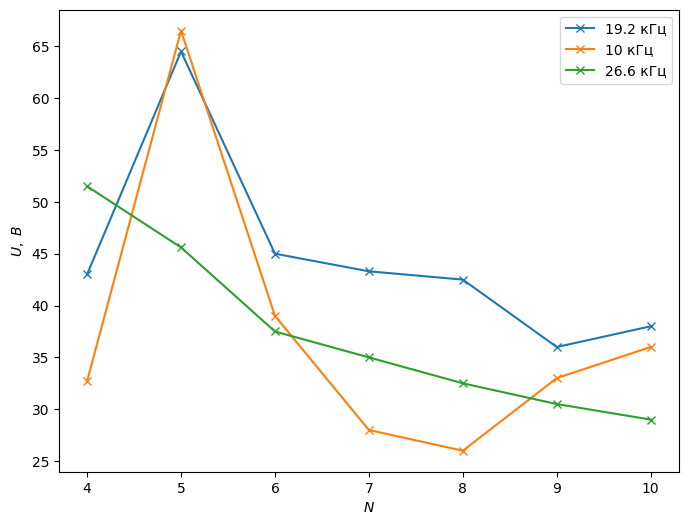
\includegraphics[width=0.7\linewidth]{plot/fig7.png}
    \caption{Зависимость амплитуды между ячейками от номера.}
\end{figure}

\section{Вывод}
Проведя исследование длинной линии и изучив изменение электрического сигнала на ее концах, мы разработали способы определения групповой и фазовой скоростей сигналов различных форм. Благодаря использованию амплитудно-частотной характеристики длинной линии, мы смогли определить ее характеристики, такие как диэлектрическая и магнитная проницаемости слоя между проводящими элементами. Преобразовав АЧХ и ФЧХ с помощью вспомогательных величин, таких как коэффициент затухания и волновой коэффициент, мы также изучили несколько способов определения удельной проводимости материала. Однако, результаты этих способов заметно отличались друг от друга, что может быть связано с ошибками в измерении амплитуды.

Кроме того, мы исследовали модель длинной линии, представленную последовательными ячейками известной ёмкости и индуктивности. Мы обнаружили, что эта модель влияет на сигнал аналогичным длинной линии образом с погрешностью порядка 20\%. Кроме того, распределение амплитуды по последовательным ячейкам модели длинной линии может соответствовать распределению в длинной линии.



\end{document}
